\documentclass{article}
\usepackage{listings}
\usepackage{hyperref}
\usepackage{graphicx}

\author{Hendrik Schick, Tobias Dorra}
\title{Project for Deep learning in medical imaging: Segmentation - MIC \\ \begin{large} 
Task 1: Obtain, Load \& Visualize Datasets
\end{large}}

\begin{document}
	
	\maketitle

	\section{Task}

		The task was to load and visualize the given datasets.

		\subsection{The datasets}

			This project focuses on two datasets, one of them is focused on the liver, the other one on the prostate. Both datasets have the same format.

			Each dataset consists out of three folders:

			\begin{description}
				\item[imagesTr] The volumetric images that shall be used for training.
				\item[labelsTr] The segmentation masks for the images in imagesTr.
				\item[imagesTs] Images for testing.
			\end{description}

			All images are in the NIfTI-1 Data format (file extension \lstinline{.nii.gz}).

	\section{Implementation}

		\subsection{Loading} \label{loading}

			We used the function \lstinline{nibabel.load()} from the python library \href{https://nipy.org/nibabel/}{nibabel} to read the image files.

			This gave us the image data in form of three dimensional numpy arrays.

			Additionaly to that, we noticed, that the resolution of the images is different allong the different axises. So we needed the correct scaling factors to display the images without distortions. Nibabel returns an affine transformation matrix alongside the pixel data, that transforms pixel-coordinates to world-space coordinates. The elements on the diagonal of this matrix is what we used as scaling factors.

		\subsection{Visualisation}

			For visualisation, the images were pre-processed using numpy and then shown using matplotlib.

			Since the images are volumetric, we decided, to show slices of the images. We extracted slices in uniform intervals, along all three axises.

			In terms of colouring, there are two options that both were implemented: 
			\begin{enumerate}
				\item Colour only based on the density value inside of the input image. We choose a colour palette, that starts at blue, progresses to red and ends at yellow, to have a better contrast compared to just showing the raw grey scale image. See figures~\ref{fig:figure1} and~\ref{fig:figure2} for examples.
				\item Just draw the image in greyscale, but overlay it with colours based on the values from the segmentation mask. See figures~\ref{fig:figure3} and~\ref{fig:figure4} for examples.
			\end{enumerate}

			\begin{figure}[tbp]
				\centering
				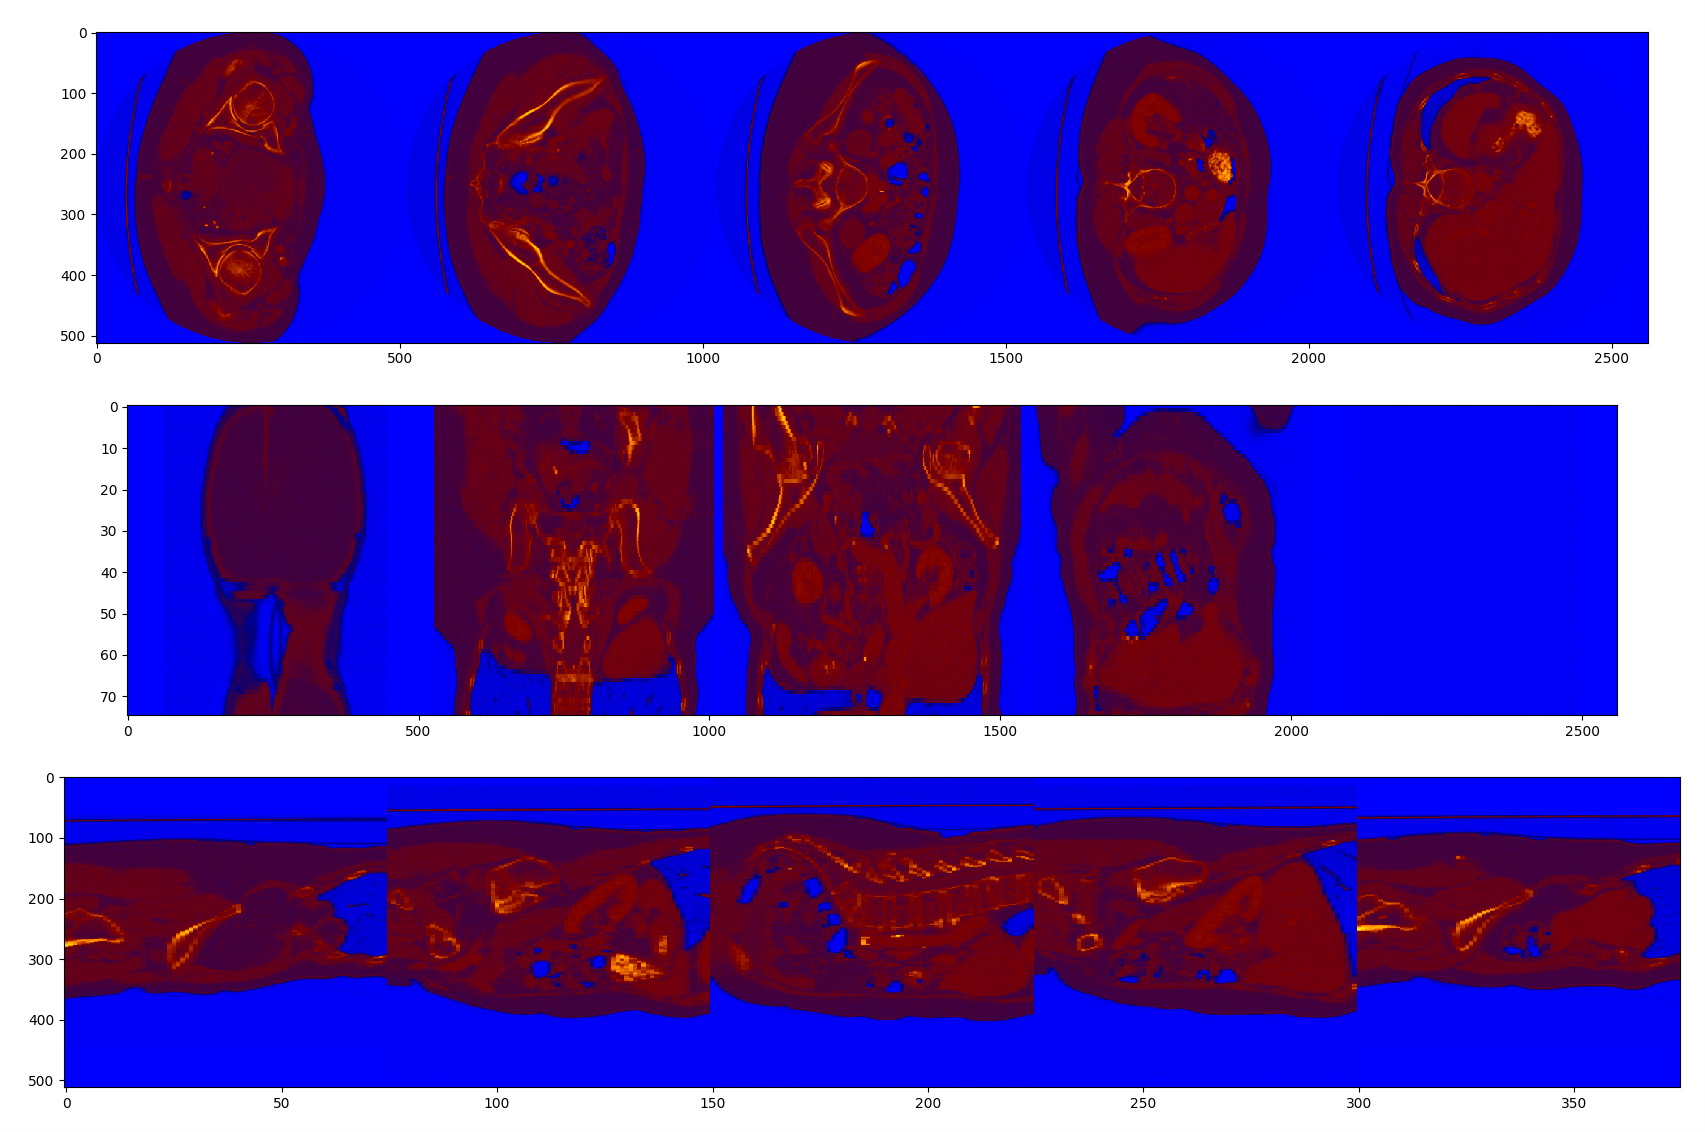
\includegraphics[width=.6\textwidth]{images/image_slices}
				\caption{Various image slices in x, y and z direction}
				\label{fig:figure1}
			\end{figure}
			\begin{figure}[tbp]
				\centering
				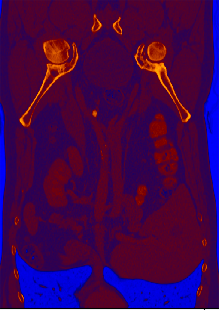
\includegraphics[width=.6\textwidth]{images/image}
				\caption{Detail: Colouring of the images}
				\label{fig:figure2}
			\end{figure}
			\begin{figure}[tbp]
				\centering
				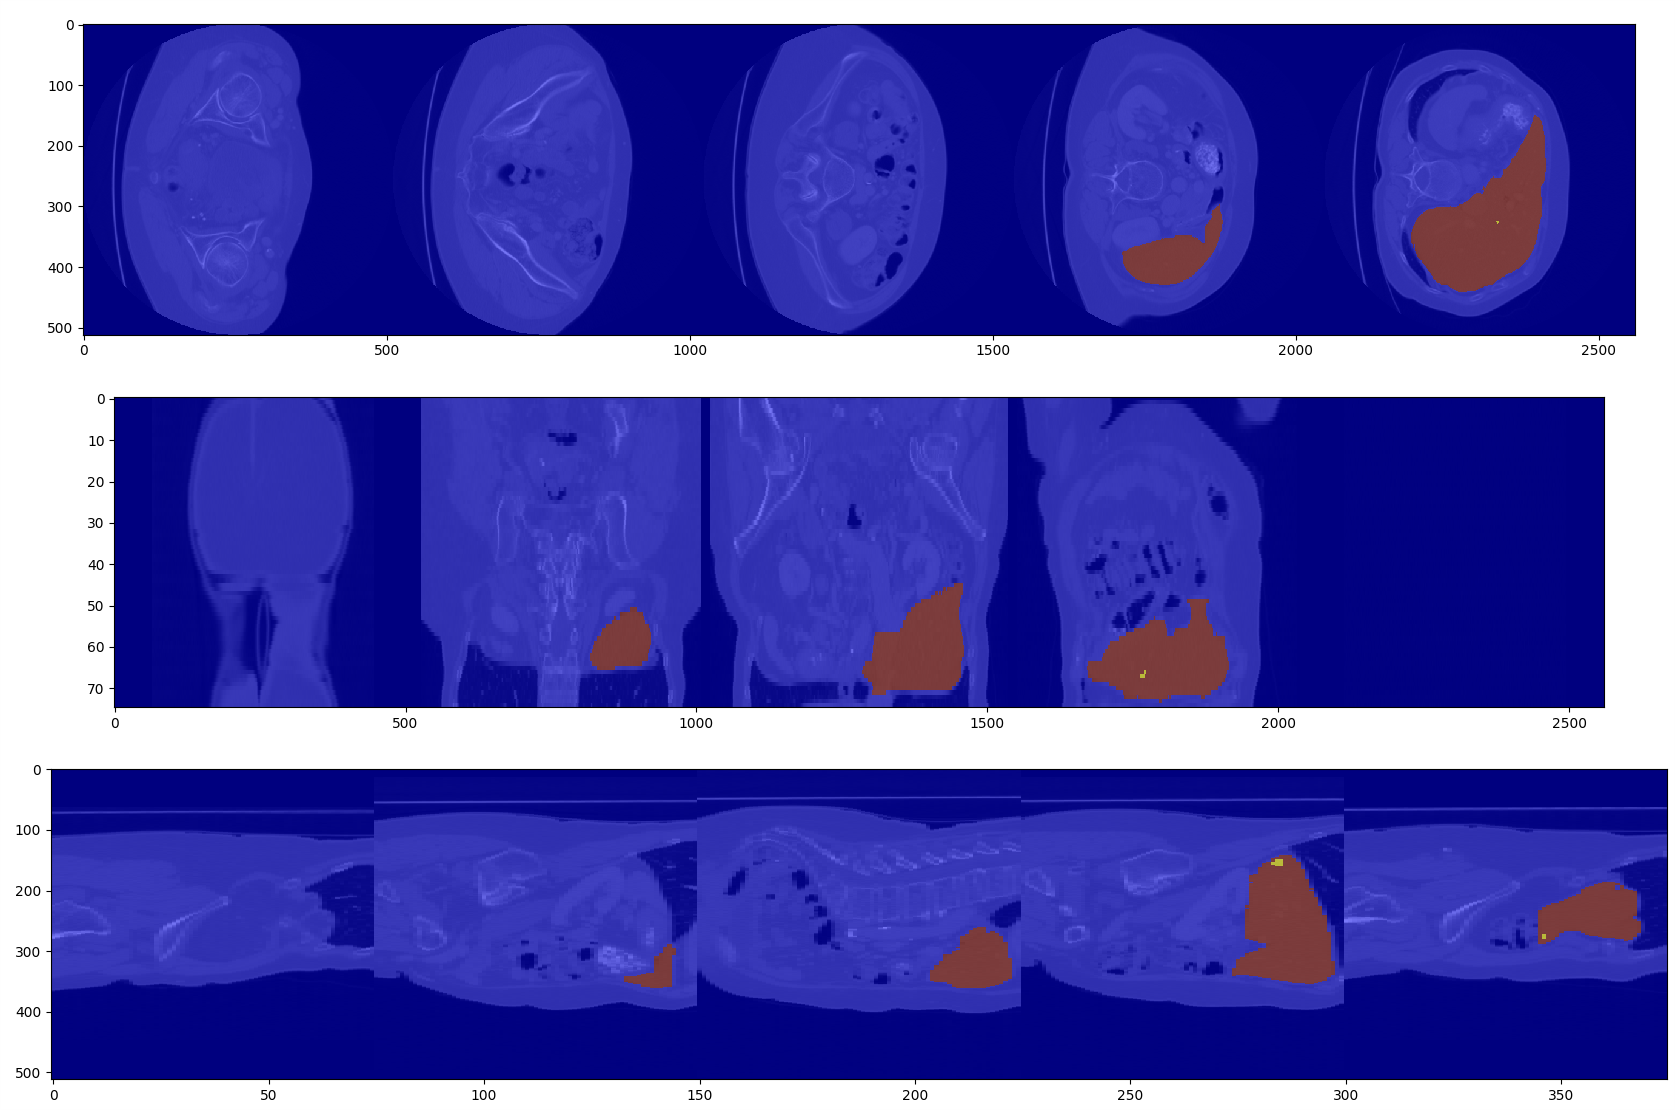
\includegraphics[width=.6\textwidth]{images/image+labels_slices}
				\caption{Various image slices in x, y and z direction with a segmentation mask}
				\label{fig:figure3}
			\end{figure}
			\begin{figure}[tbp]
				\centering
				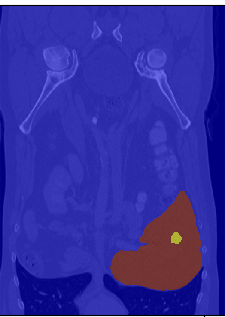
\includegraphics[width=.6\textwidth]{images/image+labels}
				\caption{Detail: Colouring of the segmentation mask}
				\label{fig:figure4}
			\end{figure}

			We also experimented with rendering the whole volume at once using the emission absorption model, instead of showing individual slices. When using the emission absorption model, each 'layer' of the image can emit some light and also absorb a part of the light that comes from the layers behind it. How much light is emitted or absorbed is controlled by the image data. You can iterate over the layers from back to front and accumulate the amount of light that leaves each layer. 

			However, the results of this were not as detailed as we hoped for, you can make out way more details in the simple slices described above, so we went with the slices-approach instead. However, you can still see an example image of how it looks in figure~\ref{fig:figure5}.

			\begin{figure}[tbp]
				\centering
				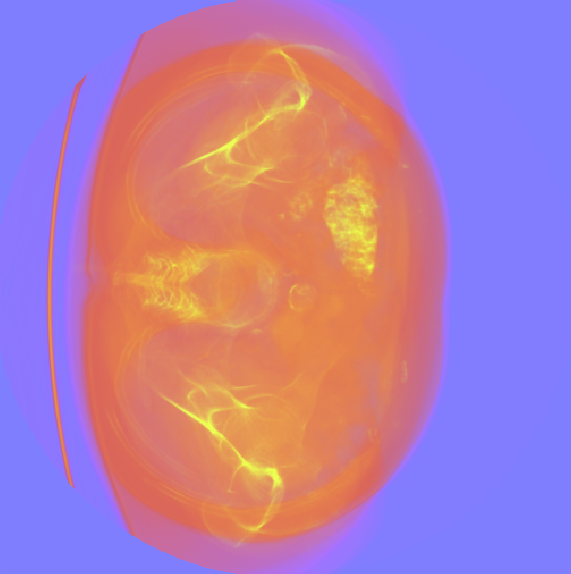
\includegraphics[width=.6\textwidth]{images/emit-absorb}
				\caption{Display of the complete volume at once using the emmission absorption model.}
				\label{fig:figure5}
			\end{figure}

	\section{Problems and future tasks}

		There were no major problems with loading or visualizing the dataset. The next step will be to use the datasets for training an actual model. Therefore, we will probably need to do some preprocessing. For the sake of visualizing the data, we just used the \lstinline{aspect} parameter of the \lstinline{imshow} function from matplotlib to account for the different image resolutions per axis mentioned in section~\ref{loading}. For training an actual model, we probably will have to actually stretch the image according to those scaling factors. Otherwise, the model would be dependant on the (x/y/z-)resolution of the images that were used for training.


\end{document}
% LIVER_PATH + TRAINING + '/liver_3.nii.gz'
